%----------------------------------------------------------------------------------------
%----------------------------------------------------------------------------------------
%----------------------------------------------------------------------------------------
%Method
%----------------------------------------------------------------------------------------
%----------------------------------------------------------------------------------------
%----------------------------------------------------------------------------------------

\section{METHOD}
\label{sec: method}
 \subsection{Self Organizing Maps}
 \label{sec: som}
 
 The SOM is a clustering method which reduces the dimension of data to lower dimensions, usually 1 or 2D, while preserving topological features of the original data.
 Results of SOM contain nodes (neurons) that arranged in 1D or 2D arrays \citep{Kohonen98}. 
 
 Each node may contain one or more samples from input data and distance between nodes represents similarity or dissimilarity of underlying samples. 
 In the way that similar data are closer together in the array and the further nodes go from each other, the more dissimilarity appears between their samples.
 A weight vector ``\boldit{W}" with same dimension of the input data associates with each node which will be changed during the process and has a key factor in a position of nodes in the map.
 
 \cite{Geach12} presented the application of the SOM and demonstrate the algorithm of the SOM in detail. In this section we are going to talk briefly about the algorithm of the SOM, how we create our maps and a test model which will help to interpret our results. 
 \subsubsection{Algorithm of SOM} 
 \label{sec: algorithm}
     Assuming we have a data set which contains vectors, \boldit{V} $\in \Re^n$, and we want to map them on S1 by S2 map. 
     We start by creating S1 $\times$ S2 empty neurons. 
     The initial arrangement of these neurons depends on a map's topology provided by users.
     In the case of the 1D maps, since each neuron has two immediate neighbours the topology of the map does not have any effect on the final result and we can choose any topology.
     However, in 2D maps, the shape of the neurons specifies the number of the immediate neighbours for each neuron and it is up to user that which shape is more suitable for their data.
     In this paper, we chose hexagonal topology which gives each neuron six neighbours, and causes more interactions between neurons.
     Then, a random weight vector, \boldit{W} $\in \Re^n$, will be assigned to each node.
     The process of creating SOM, happens over series of $N$ iterations. 
     During each iteration the weight vectors might change according to the Kohonen learning rule (equation~\ref{equ: weight adj}). 
      In each iteration SOM code:
     \begin{enumerate}
        \item Chooses a random vector from our data set ($V_i$).
        \item Calculates the Euclidean distance for each node, $j$, as  $D_j^2= \sum_{i=0}^{i=n} (V_i - W_i)^2$, and finds a neuron with minimum $D_j$, (``$D_{j_{min}}$"). This neuron is the winner node and is called the Best Matching Unit (BMU). 
        \item  Computes the radius of the neighbourhood of the BMU to find nodes within this radius. The weight vectors of these nodes will be affected in the next steps. This value is arbitrary and initially can be set to be as high as half of the SOM size and then it decades exponentially over each iteration:
        \begin{equation}
            r^t_{BMU} = r^0_{BMU}e^{(-t/\tau)}
        \end{equation}
        where $\tau$ is a decay constant and usually set to be the same as the number of iterations, $N$. $r^0_{BMU}$ and $r^t_{BMU}$ is the radius of the neighbourhood at 0th and $t$th iteration, respectively. 
        \item Changes the weight vectors of the BMU, and all the nodes within $r^t_{BMU}$ as:
        \begin{equation}
            \label{equ: weight adj}
            w(t+1)=w(t)+L(t) \times R(t) \times(v(t)-w(t))
        \end{equation}
        where $L(t) = L_0 e^{(-t/\tau)}$ is the learning factor which prevents divergence of the SOM and $R(t)=\exp(-\frac{D_j^2}{2r^t_{BMU}})$ is the influence rate. $R(t)$ determines how the weight of nodes in the neighbourhood of BMU will change.
        \item  Repeats these steps for $N$ times.
     \end{enumerate}
     
\subsection{Creating SOM}
\label{sec: create_som}
     In order to create SOM, we used {\tiny MATLAB} neural network 
     toolbox~\citep[NNT,][]{matlabtolbox}.
     %%Sr160611: Last time I got the following note from the MNRAS editor:
     %"Please note that computer software/programming lan- guages must be styled in SMALL CAPITAL LETTERS, according to journal style. Please check and correct this paper accordingly."
     SOM in {\tiny NNT} can be created by {\tiny NEWSOM} or {\tiny SELFORGMAP} library which both work in two phases. 
     Phase one is the ``ordering phase". 
     This phase starts with maximum neighbourhood distance, and initial high learning factor usually 0.9 which is provided by the user. 
     The ordering phase continues for the requested number of iterations.
     During the iterations, the learning factor reduces to tuning phase leaning factor and the neighbourhood distance reaches to tuning phase neighbourhood distance which both of the numbers set by the user.
     In the ordering phase, the changes in the learning factor and the neighbourhood distance adjust with the number of the iterations, in the way that at the last iteration, these two values reach to the initial values for the second phase.
     
     The second phase is the ``tuning phase".
     In this phase the neighbourhood distance is at its minimum, but learning factor decreases very slowly.
     This minimum neighbourhood distance and slowly decreasing the leaning factor helps to fine tune the topology results and causes the more stable SOM. 
     The number of iterations in this tuning phase most be much more than the number iterations in ordering phase, to allow the tuning to happen slowly. %cite kohenen book?!
     We chose the number of epochs the tuning phase to be 3 times more than the number of epochs in the ordering phase.
     
     To show our results, we used two of the {\tiny NNT}'s built-in plots.
     These plots, which are evolved version of old SOM plots, are designed to show distance between each clusters more clear.
     A Hits map, which shows the number of the times each neuron become the winner (hits), and a distance map, which shows the same neurons as the hits map and the distance between them.
     In the maps, the purple hexagonal shape areas represent the neurons.
     The distances in a distance map are shown by the grey cycle colours.
     The darker colour represents the larger distance between neurons; whilst the lighter colours means there is a small distance between neurons.
     In hit maps, neurons with zero hit left empty.
      
    Size of SOM maps is arbitrary and there is no rules or restrictions on choosing the size of the maps. 
    Although \cite{Vesanto05} suggested that the total number of  $5\sqrt{n}$ neurons provides the most sufficient size, users usually choose the size of grids based on their data set and their usages of the results.

   
\subsection{Mock sample}
 
         \begin{figure}
            \begin{subfigure}[b]{0.5\textwidth}
                \centering
                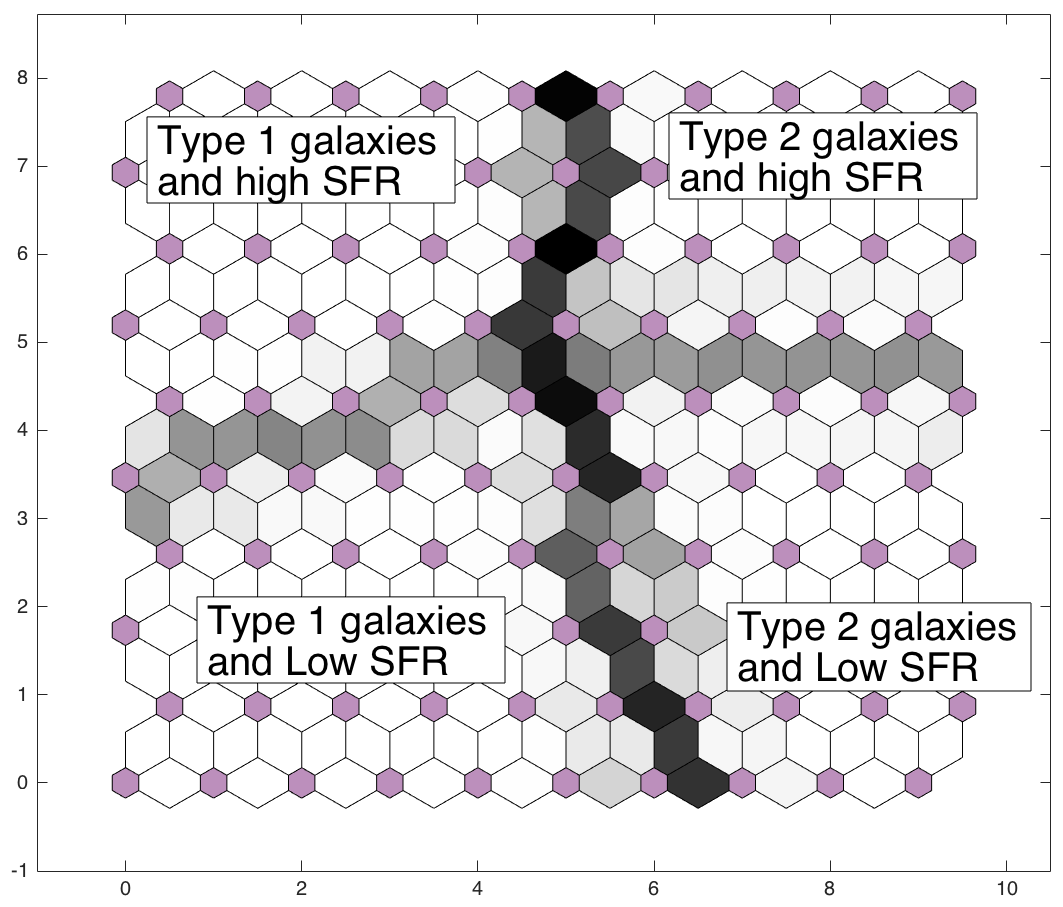
\includegraphics[width=\textwidth]{../images0.01/sample/sample2_dist.png}
            \end{subfigure}
            \hfill
            \begin{subfigure}[b]{0.5\textwidth}
                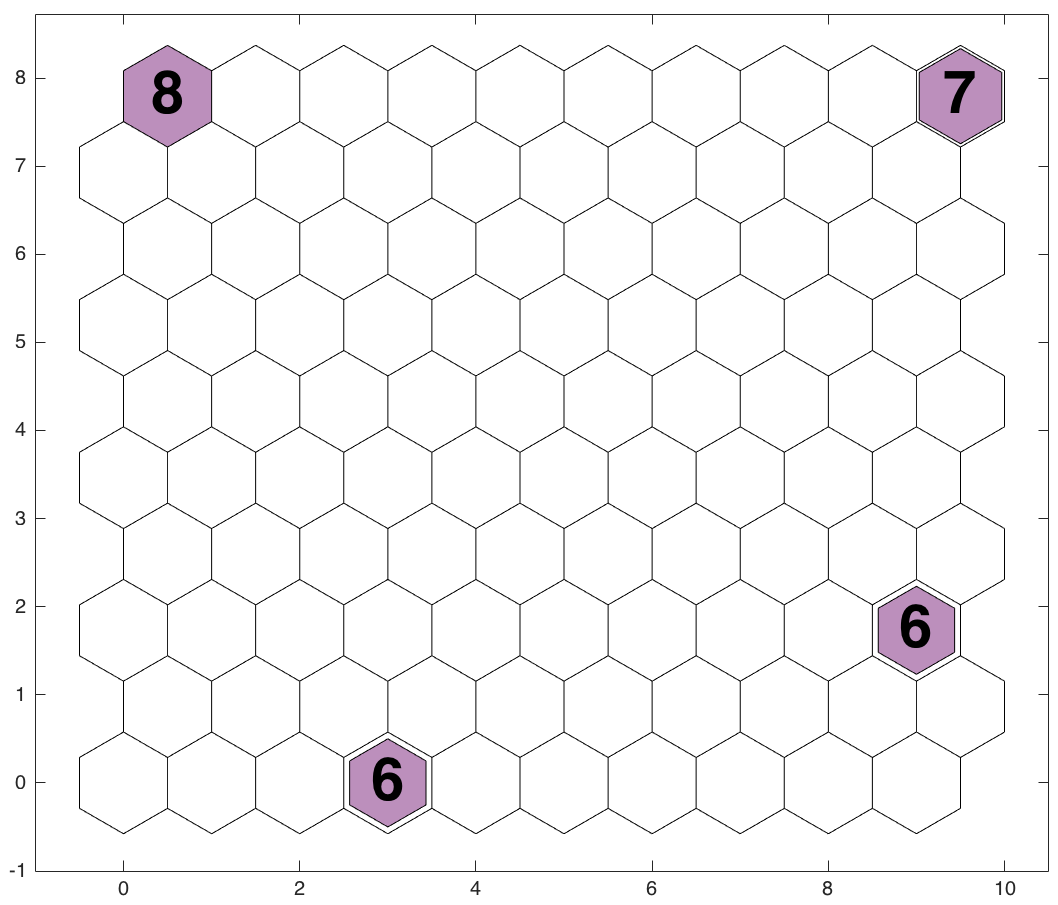
\includegraphics[width=\textwidth]{../images0.01/sample/sample2_hits.png}
            \end{subfigure}
            \caption{SOM of the mock sample. In both plots axis shows the position of the neurons. Hexagonal shapes represent the neurons. The upper plot is a distance map. The grey cycle colours show the differences between weight of each neuron with white is the minimum differences and black has the maximum one. The lower plot is a hit plot. It represents the number of samples in each neuron, while the empty with neurons means zero hit. In this sample the 27 galaxies clustered in 4 groups of 8, 7, 6 and 6 galaxies.}
            \label{fig: sample}
        \end{figure}
 
 We created  a mock sample of 27 galaxies to show how this method works, illustrate the results of SOMs, and how they can be analysed.
 The mock sample contains two information from each galaxy; The type of galaxies: type 1 or type 2, and either they are high or low star forming galaxies. 
 We generated a SOM with the size of $10 \times 10$ using the same initial values mentioned in the Section ~\ref{sec: create_som}.

 Fig. ~\ref{fig: sample} shows the SOM of the mock sample. 
 The upper plot is a distance map. 
 The axis show the position of the neurons in a $10 \times 10$ network.
 The lower plot in the Fig.~\ref{fig: sample} shows a hit map.
 On this map similar to the distance map the axis shows the position of the neurons where the hexagonal shapes are the neurons.
 The purple neurons with a number on them shows the number of galaxies in them.
 Colour coverage of neurons is different and depends on the number of the hits on the sample.
 The neuron with the maximum number of hits is completely coloured while the empty neurons are white.
 
Using this method, as we predicted, we were able to divide the mock sample galaxies into 4 distinct groups: Type 1 with high SFR, type 1 with low SFR, type 2 with high SFR and type 2 with low SFR. 
The upper plot in the Fig.~\ref{fig: sample}, clearly shows this division.
In that plot, the upper part belongs to high star forming galaxies, while the lower part belongs to the low star forming galaxies.
The left part of the plot, is where type 1 galaxies belong to and the right side is for type 2 galaxies.
Grey to black colours shows the border between regions.
The lower plot in Fig.~\ref{fig: sample} shows only 4 neurons out of 100 were occupied. 
8 galaxies are type 1 galaxies with high SFR, 7 are type 2 galaxies with high SFR, 6 are type 1 galaxies with low SFR and the other 6 are type 2 galaxies with low SFR. 
Since the input data are so simple, each entry only could get either 0 or 1 as a type of galaxy and 0 or 0.5 as an indicator of  high or low SFR, only four of the neurons were filled.

We can conclude that although each galaxy had enough space to occupy any of the neurons in the network, because of the similarity of values they stayed only in four groups.
This network is considered as a train network, and if there are any data set with similar entries, we can use this network to cluster the new data set.

As we show in the following sections, in the real world with the real data, we never have two galaxies with exactly the same information, we have more than 2 dimensions, and more galaxy types. 
Therefore, if the network has high enough neurons, the input data would eventually separate from each other and cluster into smaller and smaller groups. 
However, if the information of the input data is very similar to each other, the number of neurons is going to be much higher than the number of input samples, to be able to separate the groups from each other. 
Therefore, it is up to the users that decide the similarity or dissimilarity between the input data based on number of neurons. 


